\documentclass[a4paper, 12pt]{scrartcl}
%
\usepackage[ngerman]{babel}
\usepackage{graphicx}
\usepackage{blindtext}
\graphicspath{{figuren/}}
%
\begin{document}
%
\section*{Gute Figuren für die Abschlussarbeit}

\begin{figure}[h]
  \centering
  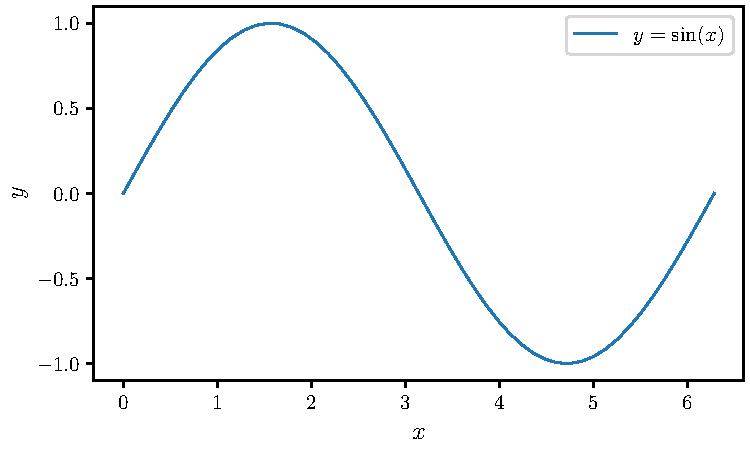
\includegraphics{sinus.pdf}
  %
  \caption{Trgonometrische Funktion $y=\sin(x)$}
\end{figure}
%
\begin{figure}[h]
  \centering
  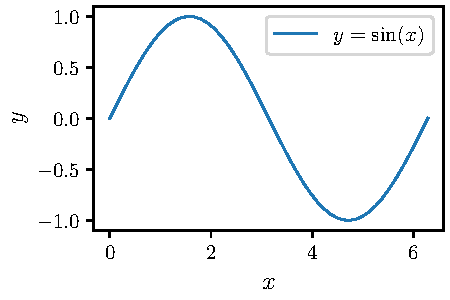
\includegraphics{sinus_small.pdf}
  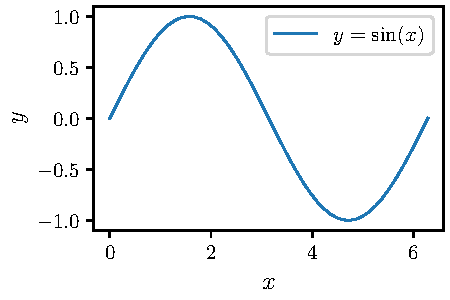
\includegraphics{sinus_small.pdf}
  %
  \caption{Trgonometrische Funktion $y=\sin(x)$}
\end{figure}
%
\begin{figure}[h]
   \centering
   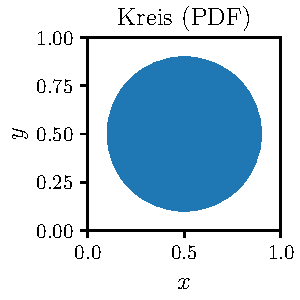
\includegraphics{kreis.pdf}
   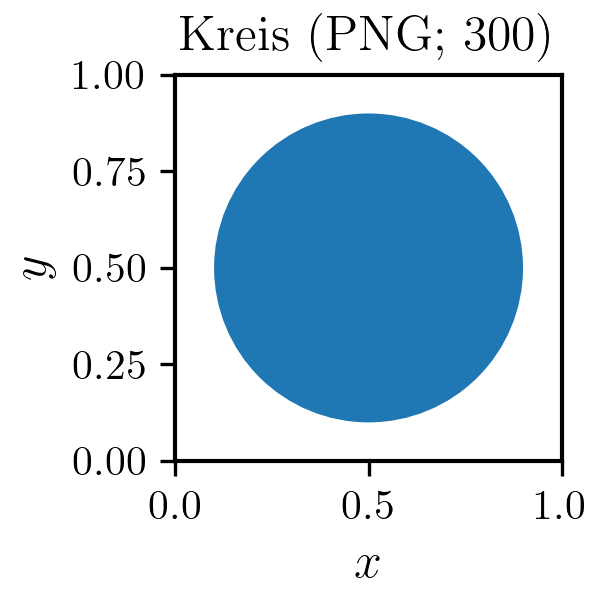
\includegraphics{kreis_300.png}
   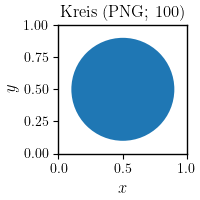
\includegraphics{kreis_100.png}
   %
   \caption{Dies ist die Unterschrift der Figur}
\end{figure}
%% %
\end{document}
%
